\documentclass[12pt]{article}

\usepackage{ amsmath, amssymb, graphicx, psfrag, bm, multirow }
\usepackage{amsmath,amsthm,amssymb}
\usepackage{mathtools}
\usepackage{tikz}
\usepackage{graphicx}
\usepackage{fancybox}
\usepackage{hyperref}
\usepackage{varwidth}
\usepackage{mdframed}
\usepackage{mathrsfs}
\usepackage[most]{tcolorbox}
\usepackage{graphicx}
\usepackage{accents}
\usepackage{listings}
\graphicspath{ {./images/} }

\addtolength{\textheight}{1.8in}
\addtolength{\topmargin}{-1.15in}
\addtolength{\textwidth}{1.5in}
\addtolength{\oddsidemargin}{-0.8in}
\addtolength{\evensidemargin}{-0.8in}
\setlength{\parskip}{0.1in}
\setlength{\parindent}{0.0in}

\pagestyle{plain}

\raggedbottom
 
\newcommand{\given}{\, | \,}
\newcommand{\lrp}[1]{\left(#1\right)}
\newcommand{\lrb}[1]{\left[#1\right]}
\newcommand{\lrc}[1]{\left\{#1\right\}}
\newenvironment{solution}{\begin{proof}[\textbf{\textit{Solution}}] }{\end{proof}}
\allowdisplaybreaks
\begin{document}

\begin{flushleft}

Prof.~David Draper \\
University of California, Santa Cruz \\
Department of Statistics \\
Baskin School of Engineering \\
Winter 2022

\end{flushleft}

\Large

\begin{center}

STAT 206 (\textsf{Applied Bayesian Statistics})

\fbox{\textbf{Take-Home Test 1}}

\large

(See updates in class and by email and \texttt{Discord} for the \textbf{final deadline}.)

\end{center}

\normalsize

\vspace*{-0.1in}

Here are the (process) ground rules: this test is open-book and open-notes, and
consists of two problems (true/false and calculation); \textbf{each of the 12
true/false questions is worth 10 points, and the calculation problem is
worth 230 total points, for a total of 350 points}.

Some advice on style as you write up your solutions: pretend that you're sitting next to the grader, having a conversation about problem $( x )$ part $( y )$. You say, ``The answer is $z$,'' and the grader says, ``Why?'' You then give your explanation, as succinctly as possible to get your idea across. The right answer with no reasoning to support it, or incorrect reasoning, will get \textbf{half credit}, so try to make a serious effort on each part of each problem (this will ensure you at least half credit). In an AMS graduate class I taught in 2012, on a take-home test like this one there were 15 true/false questions, worth a total of 150 points; one student got a score of 92 out of 150 (61\%, a D$-$, in a graduate class where B$-$ is the lowest passing grade) on that part of the test, for repeatedly answering just ``true" or ``false" with no explanation. Don't let that happen to you.  

On non-extra-credit problems, the graders and I mentally start everybody out at $-0$ (i.e., with a perfect score), and then you accumulate negative points for
incorrect answers and/or reasoning, or parts of problems left blank. On
extra-credit problems, the usual outcome is that you go forward (in the
sense that your overall score goes up) or you at least stay level, but
please note that it's also possible to go backwards on such problems (e.g.,
if you accumulate $+3$ for part of an extra-credit problem but $-4$ for the
rest of it, for saying or doing something egregiously wrong).

This test is to be entirely your own efforts; do not collaborate with
anyone or get help from anyone but me or our TA (Jacob Fontana). The intent is that the course lecture notes and readings should be sufficient to provide you with all the guidance you need to solve the problems posed below, but you may use other written materials (e.g., the web, journal articles, and books other than those already mentioned in the readings),
\textbf{provided that you cite your sources thoroughly and accurately}; you
will lose (substantial) credit for, e.g., lifting blocks of text directly
from \texttt{wikipedia} and inserting them into your solutions without full
attribution.

If it's clear that (for example) two people have worked together on a part
of a problem that's worth 20 points, and each answer would have earned 16
points if it had not arisen from a collaboration, then each person will
receive 8 of the 16 points collectively earned (for a total score of 8 out
of 20), and I reserve the right to impose additional penalties at my
discretion. If you solve a problem on your own and then share your solution
with anyone else, you're just as guilty of illegal collaboration as
the person who took your solution from you, and both of you will receive
the same penalty. This sort of thing is necessary on behalf of the many
people who do not cheat, to ensure that their scores are meaningfully
earned. In the AMS graduate class in 2012 mentioned above, five people failed the class because of illegal collaboration; don't let that happen to you.

In class I've demonstrated numerical work in \texttt{R}; you can (of course) make the calculations and plots requested in the problems below in any environment you prefer (e.g., \texttt{Matlab}, ...). To avoid plagiarism, if you end up using any of the code I post on the course web page or generate during office hours, at the beginning of your Appendix (see below) you can say something like the following:

\begin{quote}

\textit{I used some of Prof.~Draper's \texttt{R} code in this assignment, adapting it as needed.}

\end{quote}

Those of You who are using \texttt{LaTeX} or some other word-processing environment to prepare Your solutions can stick quote blocks below each question, into which You can type Your answers (I suggest that You use bold or italic font to distinguish Your solutions from the questions). If You're submitting Your answers in longhand, which is perfectly acceptable, You can just write them out on separate sheets of paper, making sure that the grader can easily figure out which chunk of text is the solution to which part of which problem.

\textbf{Please collect \{all of the code you used in answering the questions  below\} into an Appendix at the end of your document, so that (if you do something wrong) the grader can more accurately give you part credit.} 

\section{True/False}

\textit{[120 total points: 10 points each]} For each statement below, say whether it's true or false; if true without further assumptions, briefly explain why it's true (and what its implications are for statistical inference); if it's sometimes true, give the extra conditions necessary to make it true; if it's false, briefly explain how to change it so that it's true and/or give an example of why it's false. If the statement consists of two or more sub-statements and two or more of them are false, you need to explicitly address all of the false sub-statements in your answer.

\begin{itemize}

%---------------Problem A-----------------------
\item[(A)]

You're about to spin a roulette wheel, which will result in a metal ball landing in one of 38 slots numbered $\Omega = \{ 0, 00, 1, 2, \dots, 36\}$; 18 of the numbers from 1 to 36 are colored red, 18 are black, and 0 and 00 are green. You regard this wheel-spinning as fair, by which You mean that all 38 elemental outcomes in $\Omega$ are equipossible. Under Your assumption of fairness, the classical (Pascal-Fermat) probability of getting a red number on the next spin exists, is unique, and equals $\frac{18 }{ 38 }$.
\begin{tcolorbox}[breakable]
    \begin{solution}
        \textbf{True}. Since this is typical Pascal-Fermat reasoning, every ball is equipossible so we can simply take the ratio of the sum of events that meet our desired condition over the sum of the total events, which is what was stated. 
    \end{solution}
\end{tcolorbox}

\newpage
%---------------Problem B-----------------------
\item[(B)]

Under the same conditions as (A), the Kolmogorov (frequentist) probability of getting a red number on the next spin exists, is unique, and equals
$\frac{ 18 }{ 38 }$.
\begin{tcolorbox}[breakable]
    \begin{solution}
        Strictly speaking this is \textbf{False}. To explain why we follow the same reasoning as we did in Case Study 1, where we were interested in the HIV status of Bob. The probability that Bob is HIV+ is undefined to a frequentist since we can't repeat Bob's existence and see the frequency at which he is HIV+. To get around this though we considered the whole population ($\mathcal{P}_{Bob}$)) of people like Bob in all relevant ways, and then asked what was the probability that a person from this population is HIV+, and then just defined the probability that Bob is HIV+ to be that. So not strictly speaking we can do that here, and in which case the statement will be true, since we can consider the all draws similar to this one in all relevant ways ($\mathcal{P}_{red}$) and see the frequency at which red was drawn. 
    \end{solution}
\end{tcolorbox}


%---------------Problem C-----------------------
\item[(C)]

Repeat (A) and (B) but removing the assumption that the wheel-spinning is fair, and not replacing it with any other assumption about the nature of the data-generating process (taking the outcomes of the wheel spins as data).
\begin{tcolorbox}[breakable]
    \begin{solution}
        If we are not conditioning on fairness then (A) is immediately \textbf{False} this is because classical probability depends on all "elemental outcomes" to be equipossible. (B) will also become \textbf{False} because $\mathbb{P}_{red}$ will no longer be defined
    \end{solution}
\end{tcolorbox}


%---------------Problem D-----------------------
\item[(D)]

In the Bernoulli sampling model, in which $( Y_i \given \theta \, \mathcal B ) \stackrel{ \textrm{\tiny IID} }{ \sim } \textrm{ Bernoulli} ( \theta )$ for $i = 1, \dots, n$ (here $n$ is a finite positive integer and $0 < \theta < 1$), the sum $s_n = \sum_{ i = 1 }^n y_i$ of the observed data values $\bm{ y } = ( y_1, \dots, y_n )$ is sufficient for inference about $\theta$, and this means that in this model You can throw away the data vector $\bm{ y }$ and focus only on $s_n$ without any loss of information whatsoever. (Note that, as usual, we're implicitly conditioning on the known value of $n$.)
\begin{tcolorbox}[breakable]
    \begin{solution}
        This is \textbf{False}. Because if we have any uncertainty about the IID Bernoulli($\theta$) sampling model assumption. Under that assumption though this becomes narrowly \textbf{True}, since we should try not to throw away data even if we have a sufficient statistic. 
    \end{solution}
\end{tcolorbox}


%---------------Problem E-----------------------
\item[(E)]

In learning how to do a good job on the task of uncertainty quantification,
it's good to know quite a bit about both the Bayesian and frequentist
paradigms, because (a) the Bayesian approach to probability ensures logical
internal consistency of Your uncertainty assessments but does not guarantee
good calibration, and (b) the frequentist approach to probability provides
a natural framework in which to see if Your Bayesian answer \textit{is}
well-calibrated.
\begin{tcolorbox}[breakable]
    \begin{solution}
        This is \textbf{True}. This is because even though the Bayesian approach to probability ensure logical internal consistency, we can take for example in CS2 a likelihood function with extremely high prior information, which will result in a posterior PDF with little to no relation to reality. This is where having the frequentist paradigm will be useful, since even though it has potential to be logically inconsistent it can be well calibrated, and this calibration we can apply to the Bayesian paradigm. 
    \end{solution}
\end{tcolorbox}


%---------------Problem F-----------------------
\item[(F)]

The Beta$( \theta \given \alpha, \beta )$ parametric family of distributions is
useful as a source of prior distributions when the sampling model is as in
(D), because all distributional shapes (symmetric, skewed, multimodal, ...)
on $( 0, 1 )$ are realizable by single members of this family.
\begin{tcolorbox}[breakable]
    \begin{solution}
        This is \textbf{False}. That is because we can't achieve a multimodal distribution. It would be \textbf{True} if you omit the multimodal part. 
    \end{solution}
\end{tcolorbox}


%---------------Problem G-----------------------
\item[(G)]

Specifying the ingredients $\{ p ( \theta \given { \mathcal B } ), p ( D \given
\theta \, { \mathcal B } ), ( { \mathcal A \given { \mathcal B } } ), U ( a, \theta \given { \mathcal B } ) \}$ in Your model for Your uncertainty about an unknown $\theta$ (in light of background information $\mathcal B$ and data $D$) is typically easy, because in any given problem there will typically be one and only one way to specify each of these ingredients; an example is the Bernoulli sampling distribution $p ( D \given \theta \, { \mathcal B } )$ arising uniquely, under exchangeability, from de Finetti's Theorem for binary outcomes.
\begin{tcolorbox}[breakable]
    \begin{solution}
        This is \textbf{False} up to the semicolon. A counter example would be our prior information uncertainty in CS1: $P(\theta = 1 \given \mathcal{B}_{Bob})$ this value changed depending on what risk factors for Bob for HIV we judge to be relevant in defining the similarity judgement that specify $\mathbb{P}_{Bob}$. So this would be true if we replace the word "easy" with "hard" since there will actually be a number of possible ways we can specify these ingredients. 
    \end{solution}
\end{tcolorbox}


%---------------Problem H-----------------------
\item[(H)]

In trying to construct a good uncertainty assessment of the form $P ( A \given
\mathcal B )$, where $A$ is a proposition and $\mathcal B$ is a proposition
of the form $( B_1 \textrm{ and } B_2 \textrm{ and } \dots \textrm{ and }
B_k )$, You should try hard not to condition on any propositions $B_i$ that
are false, because that would be the probabilistic equivalent of dividing
by zero.  
\begin{tcolorbox}[breakable]
    \begin{solution}
        This is \textbf{True}. This is clear from the definition of conditional probability,
        \[P(A \given  B) = \begin{cases}\dfrac{P(A \text{ and } B)}{P(B)}  & P(B) > 0 \\ undefined & P(B) = 0 \end{cases}\]
        \end{solution}
\end{tcolorbox}


%---------------Problem I-----------------------
\item[(I)]

The kind of objectivity in probability assessment sought by people like
Venn, in which all reasonable people would agree on the assessed value, is
often impossible to achieve, because all such assessments are conditional
on the (1) assumptions, (2) judgments and (3) background information of the
person making the probability assessment, and different reasonable people
can differ along any of those three dimensions.
\begin{tcolorbox}[breakable]
    \begin{solution}
        This is \textbf{True}. What Venn and other were trying to achieve may be noble, it was still impossible. Since in their paradigm they are simply tucking away the subjectivity. Their assumptions and judgments are more clear when we consider the population when we have to choose our population under the idea of  "similar in all relevant ways". Meaning all probability models are subjective. 
    \end{solution}    
\end{tcolorbox}

%---------------Problem J-----------------------
\item[(J)]

When making a decision in the face of uncertainty about an unknown $\theta$, after specifying Your action space $( { \cal A } \given { \cal B } )$ and utility function $U ( a, \theta \given { \cal B } )$ and agreeing on the convention that large utility values are to be preferred over small ones, the optimal decision is found by maximizing $U ( a, \theta \given { \cal B } )$ over all $a \in ( { \cal A } \given { \cal B } )$.
\begin{tcolorbox}[breakable]
    \begin{solution}
        This is \textbf{False}. This is due to $\theta$ being unknown, therefore the utility function $U(a,\theta\given \mathcal{B})$ is a random variable. This can be made \textbf{True} by estimating $\theta$.
    \end{solution}
\end{tcolorbox}


%---------------Problem K-----------------------
\item[(K)]

One reason that Bayesian inference was not widely used in the early and middle parts of
the 20th century was that approximating the (potentially high-dimensional)
integrals arising from this approach was difficult in an era when computing
was slow and the Laplace-approximation technique had been forgotten.
\begin{tcolorbox}[breakable]
    \begin{solution}
        This is \textbf{True}. The reason being from the information given to us during lecture Feb 9th, which mentioned how even if we wanted to do Bayesian methods in say 1925 we'd have a hard time doing so with a $k$-dimensional vector when $k$ is greater than about 2 or 3 since we wouldn't be able to compute those integrals!
    \end{solution}
\end{tcolorbox}


%---------------Problem L-----------------------
\item[(L)]

Jaynes (2003, pp.~21--22) makes a useful distinction between
\{reality\} (epistemology) and \{Your current information about reality\}
(ontology); this distinction is useful in probabilistic modeling because
\{the world\} does not necessarily change every time \{Your state of
knowledge about the world\} changes.
\begin{tcolorbox}[breakable]
    \begin{solution}
        This is \textbf{False}. This is because reality is not epistemology and Your current information about reality is not ontology. To remedy this though we simply need to swap them and this will be true.
    \end{solution}
\end{tcolorbox}


\end{itemize}

\section{Calculation}

\begin{itemize}

\item[(A)]

\textit{[100 total points]} Consider the HIV screening example we looked at in Case Study (CS) 1, in which $( \theta = 1 )$ = (the patient is HIV positive) and $( y_1 = 1 )$ = (the blood test says the patient is HIV positive), but let's make two changes: the time is now 1985, when the first \textit{enzyme-linked immunosorbent assay (ELISA)} blood test was approved in the U.S.~for use in detecting HIV, and You now work for the Red Cross (RC), which maintains a blood bank (from which units of blood for surgeries in hospitals are drawn) and which is extremely interested in not letting HIV into their blood supply. Continuing to use CS 1 notation, let $\alpha = P ( \theta = 1 \given \mathcal{ B } )$ be the prevalence of HIV in people whose background risk factors are summarized in $\mathcal{ B }$; and let $\beta = P ( y_1 = 1 \given \theta = 1 , \, \mathcal{ B } )$ and $\gamma = P ( y_1 = 0 \given \theta = 0 , \, \mathcal{ B })$ be the sensitivity and specificity, respectively, of the first \textit{ELISA} test (let's call it $E_1$). According to Chappel, Wilson and Dax (2009, \textit{Future Microbiology}, \textbf{8}, 963--982), $( \beta, \gamma ) = ( 0.99, 0.95 )$ for $E_1$, so the first test had decent sensitivity but did not reach the same performance level in specificity. Poking around on \texttt{www.census.gov}, You'll find that the population of the United States in 1985 consisted of about 238 million people, of whom about $N = 175$ million people were 18 years old or older; let's assume that HIV is concentrated entirely in the 18+ subpopulation (which is true to a good approximation). 

The basic $( 2 \times 2 )$ table for disease screening, in the notation of this problem, is given in Table \ref{t:basic-screening-table}. \textbf{Warning:} Many published sources use the rows-and-columns convention in Table \ref{t:basic-screening-table}, but some reverse this, with rows for truth and columns for what the screening test says; an example of the latter convention is at 

\hspace*{0.25in} \texttt{https://en.wikipedia.org/wiki/Sensitivity\_and\_specificity} . 

The definitions of the four probabilities in the body of the table are as follows: $( TP, FP, FN,$ $TN )$ = \{true positive (upper left cell), false positive (upper right), false negative (lower left), true negative (lower right)\}.

\begin{table}[t!]

\centering

\caption{\textit{The basic disease screening $( 2 \times 2 )$ table on the probability scale, with $\theta = ( 1$ if the disease is truly present, 0 otherwise), $y_1 = ( 1$ if the screening test says the disease is present, 0 otherwise), and $( \alpha, \beta, \gamma )$ = (prevalence, sensitivity, specificity).}}

\label{t:basic-screening-table}

\bigskip

\begin{tabular}{cc|c|c|c}

& \multicolumn{1}{c}{} & \multicolumn{2}{c}{\textbf{Truth}} \\

& \multicolumn{1}{c}{} & \multicolumn{1}{c}{HIV \textcircled{+} $( \theta = 1 )$} & \multicolumn{1}{c}{HIV \textcircled{$-$} $( \theta = 0 )$}  & Total \\ \cline{3-4}

\textbf{Blood} & \textcircled{+} $( y_1 = 1 )$ & $TP \! : \, \alpha \, \beta$ & $FP \! : \, ( 1 - \alpha ) \, ( 1 - \gamma )$ & $\alpha \, \beta + ( 1 - \alpha ) \, ( 1 - \gamma )$ \\ \cline{3-4}

\textbf{Test} & \textcircled{$-$} $( y_1 = 0 )$ & $FN \! : \, \alpha \, ( 1 - \beta )$ & $TN \! : \, ( 1 - \alpha ) \, \gamma$ & $\alpha \, ( 1 - \beta ) + ( 1 - \alpha ) \, \gamma$ \\ \cline{3-4}

& \multicolumn{1}{c}{Total} & \multicolumn{1}{c}{$\alpha$} & \multicolumn{1}{c}{$( 1 - \alpha )$} & 1

\end{tabular}

\end{table}

\begin{itemize}
%--------------------------------------------------------2A-------------------------------------------------------------------
\item[(i)]

Where did the four entries in the body of Table \ref{t:basic-screening-table} (not the margins) come from? As an example, by making an easy probability calculation, briefly explain why the upper-left entry is  $\alpha \, \beta$; why the same logic applies to the lower-right entry; and how the other entries are then immediately calculated. \textit{[15 points]}
\begin{tcolorbox}[breakable]
    \begin{solution}
        In terms of probability the \textbf{top left corner} is saying,
        \[P(\theta = 1, y_1 = 1 \given \mathcal{B})\]
        which is an \textit{and} probability and we know the form for caclulating it would be the following,
        \begin{align}
            P(\theta = 1, y_1 = 1 \given \mathcal{B}) = P(\theta = 1 \given \mathcal{B}) \cdot P(y_1 = 1 \given \theta = 1, \mathcal{B}) 
        \end{align}
        Now recall we calculate the prevelance $\alpha$, as,
        \[\alpha = P(\theta = 1\given \mathcal{B})\]
        which we see is needed in the first part of (1). We also calculate sensitivity $\beta$, as,
        \[\beta = P(y_1 = 1 \given \theta = 1, \mathcal{B})\]
        which is also needed in (1). All this together means,
        \[P(\theta = 1, y_1 = 1 \given \mathcal{B}) =  P(\theta = 1 \given \mathcal{B}) \cdot P(y_1 = 1 \given \theta = 1, \mathcal{B}) = \alpha \beta\]
        demonstrating why the upper left entry is calculated as $\alpha\beta$.

        Now for the \textbf{bottom right corner}, in terms of probability calculations it is saying,
        \[P(\theta = 0, y_1 = 1 \given \mathcal{B})\]
        which like before can be calculated as,
        \begin{align}
            P(\theta = 0, y_1 = 1 \given \mathcal{B}) = P(\theta = 0 \given \mathcal{B})\cdot P(y_1 = 0\given \theta = 0, \mathcal{B})
        \end{align}
        We see then that $P(\theta = 0 \given \mathcal{B})$ is the opposite of prevlance, meaning under law of total probability we have $P(\theta = 0 \given \mathcal{B}) = (1 - \alpha) $. Now recall how specificity is defined,
        \[\gamma = p(y_1 = 0\given \theta = 0, \mathcal{B})\]
        which is the last thing we need for (2). So putting it all together we get,
        \[P(\theta = 0, y_1 = 1 \given \mathcal{B}) = P(\theta = 0 \given \mathcal{B})\cdot P(y_1 = 0\given \theta = 0, \mathcal{B}) = (1-\alpha)\gamma\] 
        demonstrating why the bottom right entry is calculated as $(1-\alpha)\gamma$

        For the \textbf{bottom left} and \textbf{top right} boxes they follow immediately from what they are asking based on the above and under the law of total probability. Like for example the left column is based on truly HIV+ people, which is why we need $\alpha$ (prevelance) in each box, therefore the right column must have $(1-\alpha)$. Then similarly for the rows we can easily fill in the rest of the cells.
    \end{solution}
\end{tcolorbox}
\newpage
\item[(ii)]

Use this table to write down explicit formulas in terms of $( \alpha, \beta, \gamma )$ for two frequently-used quantities in disease screening that we haven't looked at yet: the \textit{positive predictive value} (PPV, also known as the \textit{precision}), $P ( \theta = 1 \given y_1 = 1, \, \mathcal{ B })$, and the \textit{negative predictive value} (NPV, with a similar interpretation for negative test results), $P ( \theta = 0 \given y_1 = 0, \, \mathcal{ B } )$, of screening tests such as $E_1$. How do the PPV and NPV relate to the \textit{false discovery} and \textit{false omission rates} (FDR = $\frac{ FP }{ FP + TP }$, FOR = $\frac{ FN }{ FN + TN }$)? Explain briefly. \textit{[20 points]}

\begin{tcolorbox}[breakable]
    \begin{solution}
        We see PPV is the probability the person is HIV+ given the test is positive and the background, and similarly NPV is the probability the person is HIV- given the test is negative and the background. Which means form PPV we are working the the top row, since the top row is the blood test reporting positive. Then to get the probability the person is HIV+ is simply taking the top left cell and dividing it by the total for the top row,
        \[\text{PPV} = P(\theta = 1 \given y_1 =1 , \mathcal{B}) = \frac{\alpha\beta}{\alpha\beta + (1-\alpha)(1-\gamma)}.\]

        By similar reasoning NPV is working with the bottom row, and we will divide the the bottom right cell by the bottom row total since the right column is the person being HIV-. Giving us,
        \[\text{NPV} = P(\theta = 0 \given y_1 = 0, \mathcal{B})= \frac{(1-\alpha)\gamma}{\alpha(1-\beta) + (1-\alpha)\gamma}.\]

        Now with how FDR and FOR relate to PPV and NPV respectively. Looking at PPV and FDR we see they are complements of one another. This is because we see for calculating denominator in the FDR we have,
        \[FP + TP = \alpha\beta + (1-\alpha)(1-\gamma)\]
        which matches the denominator of the PPV. Now the reason they are complements of one another is because for the numerator of FDR we are taking the top right cell (HIV- / FP) and PPV is taking the top left cell (HIV+ / TP), but they're both over the same row total (conditioning on the same thing). In other words we can define them in terms of one another (push \& pull),
        \[PPV = 1 - FDR.\]
        By similar reasoning we have the same relation for NPV and FOR,
        \[NPV = 1 - FOR.\]


    \end{solution}
\end{tcolorbox}
\newpage
\item[(iii)]

The Centers for Disease Control and Prevention (CDC, not CDCP, for some reason) estimated in 2016 that the U.S.~prevalence of HIV in 1985 was based on about 500,000 cases, for a prevalence rate in the 18+ subpopulation of $\frac{ 500000 }{ 175000000 } = \alpha^* \doteq 0.00286$, about 0.3\% (roughly the same as the U.S.~prevalence rate today). The Red Cross (RC) would not have been privy to this information in 1985, but assuming that HIV status and the blood-donation choice mechanism are independent, which is almost certainly upper-bounding for $\alpha$, would give $\alpha^*$ as the RC prevalence. Use this value for $\alpha$ and the $( \beta, \gamma )$ values for $E_1$ to compute the PPV, NPV, FDR and FOR values defining the blood-screening real-world environment facing the RC in 1985. Would You say that $E_1$ was highly successful at keeping HIV out of the RC blood supply in 1985? Explain briefly. \textit{[25 points]}

\begin{tcolorbox}[breakable]
    \begin{solution}
        Calculating with $(\alpha, \beta, \gamma ) = (0.00286, 0.99, 0.95)$. Using these values, the equations from the previous values and calculating them in R we get,
        \begin{center}
            \begin{tabular}{ |c|c| } 
             \hline
             PPV & 0.054 \\
             \hline
             NPV & 0.999 \\ 
             \hline
             FDR & 0.946 \\ 
             \hline 
             FOR & 0.00003\\
             \hline
            \end{tabular}
            \end{center}
            I would say that $E_1$ was indeed highly successful at keeping HIV out of the RC blood supply in 1985. This can be seen by the extremely high NPV, meaning that when someone tested negative under $E_1$ it was \textbf{extremely} likely they were indeed negative. This was at the cost though of throwing out clean blood due to the FDR being so high. This is the best compromise to have though since our priority is keeping HIV blood out of the RC blood supply. 
    \end{solution}
\end{tcolorbox}

\item[(iv)]

Holding $( \beta, \gamma )$ at the $E_1$ values and varying $\alpha$ from 0 to (say) $10 \, \alpha^*$, plot the PPV and NPV as functions of $\alpha$. How sensitive were each of these quantities to prevalence in the 1985 RC environment? Explain briefly. \textit{[15 points]}

\begin{tcolorbox}[breakable]
    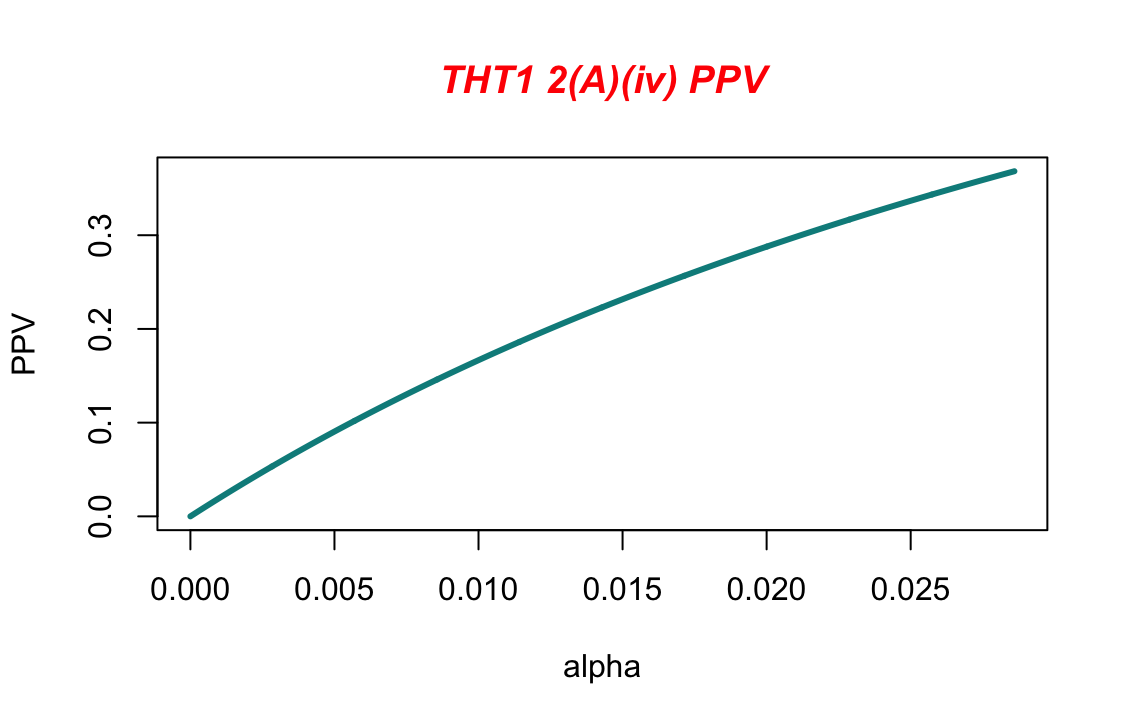
\includegraphics[scale = 0.18]{ppv} 
    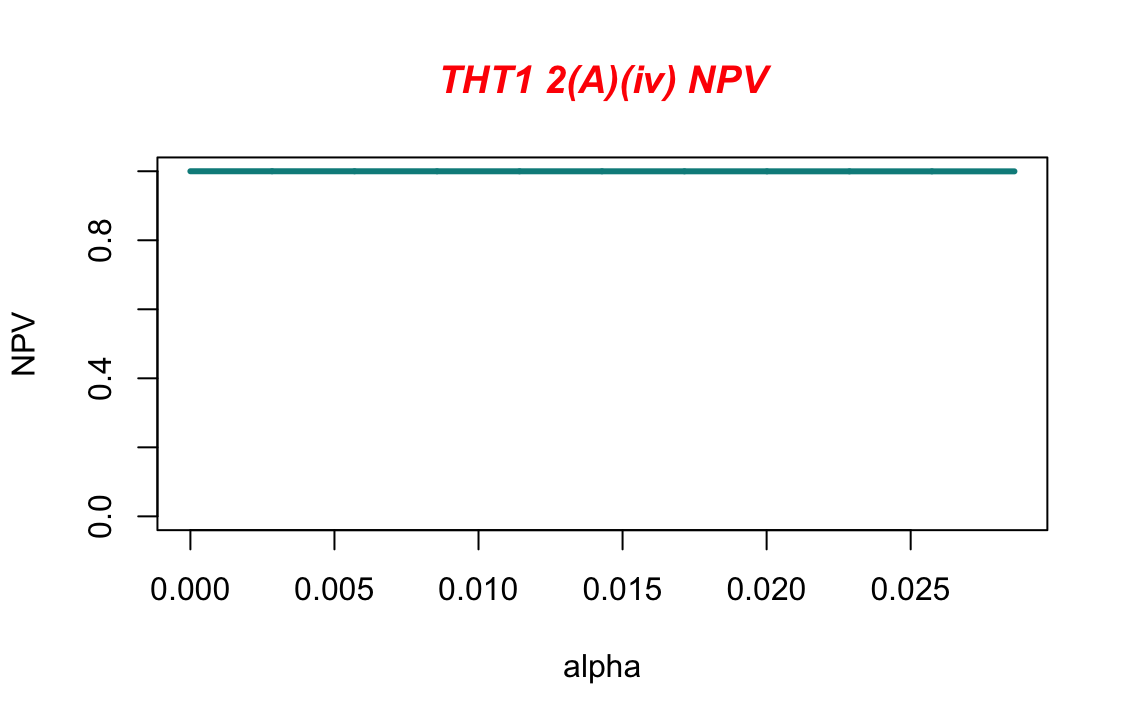
\includegraphics[scale = 0.18]{NPV1} \\
    From these graphs we can see that the PPV is indeed sensitive to $\alpha$ since our PPV ranges from about 0 percent all the way to 40 percent. Meaning the PPV could be more accurate, but it would mean for HIV to be more prevalent in the population. Opposite to the PPV though we see that the NPV is affected very little by the change in alpha, it still maintains a very high accuracy from 0 to $10\alpha^{*}$.
 \end{tcolorbox}

\end{itemize}
\newpage

\begin{table}[t!]

\centering

\caption{\textit{Partially-filled-out table of expected numbers of people receiving HIV diagnoses under the Congressperson's plan.}}

\label{t:congressperson-table}

\bigskip

\begin{tabular}{cc|c|c|c}

& \multicolumn{1}{c}{} & \multicolumn{2}{c}{\textbf{Truth}} \\

& \multicolumn{1}{c}{} & \multicolumn{1}{c}{HIV \textcircled{+} $( \theta = 1 )$} & \multicolumn{1}{c}{HIV \textcircled{$-$} $( \theta = 0 )$}  & Total \\ \cline{3-4}

\textbf{Blood} & \textcircled{+} $( y_1 = 1 )$ & 495,000 & $ 8,725,000$ & $9,220,000$ \\ \cline{3-4}

\textbf{Test} & \textcircled{$-$} $( y_1 = 0 )$ & $5,000$ & $165,775,000$ & $165,780,000$ \\ \cline{3-4}

& \multicolumn{1}{c}{Total} & \multicolumn{1}{c}{$500,000$} & \multicolumn{1}{c}{174,500,000} & $175,000,000$

\end{tabular}

\end{table}

Shortly after $E_1$ was approved in 1985, a member of the U.S.~Congress made a speech on the floor of the House of Representatives expressing the opinion that HIV was such a serious public health threat that everyone 18+ years old should be tested with $E_1$. The goal in this final part of the problem is to fill out a new version of Table \ref{t:basic-screening-table} with numbers quantifying what would have happened to the $N = 175$ million Americans under this Congressperson's plan. If we knew for sure that $\alpha = \alpha^*$, we could just use that value of $\alpha$ and the already-established values of $( \beta, \gamma )$, and multiply all of the resulting entries in Table \ref{t:basic-screening-table} by $N$, but we don't know that for sure. Consider $\alpha$ an unknown quantity (in STAT 131 we would have called it a random variable) with expected value $E ( \alpha \given \mathcal{ B } ) = \alpha^*$. 

\begin{itemize}

\item[(v)] 

By looking at the form of all 9 of the entries in Table \ref{t:basic-screening-table} (including the margins) as functions of $\alpha$ (and remembering basic properties of expectation from STAT 131), briefly explain why we can obtain a table of \textit{expected} cell and margin counts just by multiplying all of the entries in Table \ref{t:basic-screening-table} by $N$ and then substituting in $( \alpha, \beta, \gamma ) = \left( \frac{ 1 }{ 350 }, 0.99, 0.95 \right)$. Complete Table \ref{t:congressperson-table} by filling in the symbolic cells and margins with the appropriate integers; I've given You a headstart on some of them. Briefly summarize the likely good and bad outcomes of the Congressperson's plan, when viewed as an instance of national health policy. (\textit{Hint:} The first Western Blot test for HIV, which was quite a bit more accurate than $E_1$, was not developed until 1987.) In Your view, would the good outcomes outweigh the bad, or the other way around, or is it hard to come to a clear judgment? Explain briefly. (Note that we're not doing a complete \textit{cost-benefit} analysis here, since we've not taken into account how much administering 175,000,000 $E_1$ tests would cost in time and money.) \textit{[25 points]}

\begin{tcolorbox}[breakable]
    \begin{solution}
        We can explain this by first considering just the top left cell, or in other words the True Positive. We know the probability of the True Positive to be,
        \[TP = P(\theta =1 , y_1 = 1 \given \mathcal{B}) = \alpha \cdot \beta\]
        now looking at it as a function of $\alpha$ we can express it as,
        \[g_{TP}(\alpha) = \alpha\cdot \beta.\]
        Taking the expected value of $g_{TP}$ we get,
        \[E\left(g_{TP}(\alpha)\given \mathcal{B}\right) = E(\alpha \cdot \beta \given \mathcal{B})\]
        we have that $\beta$ is fixed and known, meaning we can pull it out and we also know the expected value of alpha given the background to be $\alpha^{*}$ we get,
        \[E(\alpha\cdot\beta \given \mathcal{B}) = \beta E(\alpha \given \mathcal{B}) =\beta \cdot \alpha^{*}. \]
        By this reasoning then to get a count we have,
        \begin{align*}
            E(N\cdot g_{TP}(\alpha) \cdot \beta\given\mathcal{B}) = E(N\alpha\beta \given \mathcal{B}) &= N\alpha^{*}\beta \\
            &= 175,000,000\cdot\frac{50,0000}{175,000,000}\cdot 0.99 \\
            &=495,000
        \end{align*}
        which is what we see in the given table. The reason we can fill the table in this way is because every cell and margin are linear functions of $\alpha$ so calculating the expectation in order to get the count it'll be the same manner as above, meaning we can just multiply by $N$.
       
        \textbf{Policy Implications:} \\
        Good: 495,000 HIV+ people would be told know they have HIV+.

        Bad: 8,725,00 people would be told they're HIV+ when they're not.

        Because a gold standard test wasn't developed until later, this would be disastrous. This is because we're telling about 9 million Americans that they have HIV when they indeed don't. 

    \end{solution}
\end{tcolorbox}

\end{itemize}


%----------------------------------------2B----------------------------------------------------
\item[(B)]

\textit{[130 total points]} (Bayesian conjugate inference with the Exponential distribution) In a consulting project that one of my Ph.D.~students and I worked on at the University of Bath in England before I came to Santa Cruz, a researcher from the Department of Electronic and Electrical Engineering (EEE) at Bath wanted help in analyzing some data on failure times for a particular kind of metal wire (in this problem, failure time was defined to be the number of times the wire could be mechanically stressed by a machine at a given point along the metal before it broke). The $n = 14$ raw data values $y_i$ in one part of her experiment, arranged in ascending order, were 
\[ 
495 \ \ \ 541 \ \ \ 1461 \ \ \ 1555 \ \ \ 1603 \ \ \ 2201 \ \ \ 2750 \ \ \
3468 \ \ \ 3516 \ \ \ 4319 \ \ \ 6622 \ \ \ 7728 \ \ \ 13159 \ \ \ 21194 
\] 
From the context $\mathbb{ C }$ of this problem, Your uncertainty about these data values before they were observed is exchangeable, which implies that it's appropriate to model the $y_i$ as conditionally IID, but from what distribution?
The simplest model for failure time data involves the \textit{Exponential} distribution: 
\begin{equation} \label{e:exponential-model-1}
( y_i \given \lambda \, \bm{ E } \, \mathcal{ B } ) \stackrel{ \mbox{\footnotesize IID} }{ \sim } \textrm{Exponential} ( \lambda ) \! : \ \ \ \textrm{i.e.,} \ \ \ p( y_i \given \lambda \, \bm{ E } \, \mathcal{ B } ) = \left\{ \begin{array}{cc} \frac{ 1 }{ \lambda } \exp( - \frac{
y_i }{ \lambda } ) & y_i > 0 \\ 0 & \mbox{otherwise} \end{array} \right\}
\end{equation}
for some $\lambda > 0$, in which $\bm{ E }$ stands for the Exponential sampling distribution assumption (which is not part of $\mathcal{ B }$, since it's not implied by problem context but has instead been chosen for simplicity). (\textbf{NB} This distribution can be parameterized either in terms of $\lambda$ or $\frac{ 1 }{ \lambda }$; whenever it comes up, You need to be careful which parameterization is in use.)

\begin{itemize}

\item[(i)]

To see if this model fits the data set given above, You can make an \textit{Exponential probability plot}, analogous to a Gaussian quantile-quantile plot (\textit{qqplot}) to check for Normality. In fact the idea works for more or less any distribution: You plot 
\begin{equation} \label{e:probability-plot-1}
y_{ ( i ) } \ \ \ \mbox{(vertical axis)} \ \ \ \mbox{versus} \ \ \ F^{ -1 } \left( \frac{ i - 0.5 }{ n }
\right) \, ,
\end{equation}
where $y_{ ( i ) }$ are the $y$ values sorted from smallest to largest and $F$ is the CDF of the distribution You're considering (the 0.5 is in the numerator to avoid problems at the edges of the data). In so doing You're graphing the data values against an approximation of \textit{what You would have expected for the data values if the CDF of the $y_i$ really had been $F$}, so the plot should resemble the 45$^\circ$ line if the fit is good.  

\begin{itemize}

\item[(a)] 

Work out the CDF $F_Y ( y \given \lambda \, \bm{ E } )$ of the Exponential$( \lambda )$ distribution (parameterized as in equation (\ref{e:exponential-model-1}) above)
and show that its inverse CDF is given by
\begin{equation} \label{e:probability-plot-2}
F_Y ( y \given \lambda \, \bm{ E } ) = p \iff y = F^{ -1 }( p \given \lambda \, \bm{ E } ) = - \lambda \, \log ( 1 - p ) \, .
\end{equation}
\textit{[10 points]} 

\begin{tcolorbox}[breakable]
    \begin{solution}
        From Stats 131 we know we can work out the CDF $F_Y ( y \given \lambda \, \bm{ E } )$ by taking the integral of the PDF in the equation (3). Meaning,
        \[F_Y(y \given \lambda \bm{E}) = \int_0^{y_i} \frac{1}{\lambda}\text{exp}(\frac{-t}{\lambda})dt = 1-e^{\frac{-y}{\lambda}}. \]

        Now if we work out the inverse CDF we get,
        \begin{align*}
            F^{-1}(p \given \lambda \bm{E}) = y \Longleftrightarrow& F(y \given \lambda \bm{E} ) = p \\
             \Longleftrightarrow& 1- \text{exp}(\frac{-y}{\lambda})=p && \text{Solving for $y$} \\
             \Longleftrightarrow& y = -\lambda \log(1-p)
        \end{align*}
        as desired. 
    \end{solution}
\end{tcolorbox}

\newpage
\item[(b)] 

To use equation (\ref{e:probability-plot-2}) to make the plot, we need a decent estimate of $\lambda$. Write down the likelihood and log-likelihood functions in this model, simplified as much as You can, and plot them (on different graphs, and with $\lambda$ ranging on the horizontal scale from 2,000 to 15,000) using the data values given above. Briefly explain why the form of Your log-likelihood function implies that $\bar{ y }$, the sample mean, is sufficient for $\lambda$ in the Exponential sampling model. Show that the maximum likelihood estimate of $\lambda$ in this model is $\hat{ \lambda }_{\mbox{\tiny MLE}} = \bar{ y }$, and use this (i.e., take $\lambda = \hat{ \lambda }$ and $p = \left( \frac{ i - 0.5 }{ n } \right)$ in equations (\ref{e:probability-plot-1}) and (\ref{e:probability-plot-2})) to make an Exponential probability plot of the 14 data values above (i.e., plot the sorted $y$ values on the vertical axis against $F^{ -1 } \left( \frac{ i - 0.5 }{ n } \given \hat{ \lambda }_{\mbox{\tiny MLE}} \, \bm{ E } \right)$, superimposing the 45$^\circ$ line on it. Informally, does the Exponential model appear to provide a good fit to the data? Explain briefly. \textit{[35 points]} 

\begin{tcolorbox}[breakable]
    \begin{solution}
        First we can take the marginal sampling distribution for $Y_i$ to obtain the joint sampling distribution for,
        \begin{align*}
            \undertilde{Y} = (Y_1, \dots Y_n) & \undertilde{y} = (y_1, \dots , y_n).
        \end{align*}
        The joint PDF will be (note that $P_{Y_i}(y_i \given \lambda \bm{E}) = \dfrac{1}{n}\text{exp}(-\dfrac{y_i}{\lambda})I_{(0,\infty)}(y_i)$) ,
        \begin{align*}
            P_{\undertilde{Y}} ( \undertilde{y} \given \lambda \bm{E}) &= \Pi_{i=1}^{n} P_{Y_i}(y_i \given \lambda \bm{E} ) \\
            &= \Pi_{i=1}^{n} \frac{1}{n}\text{exp}(-\frac{y_i}{\lambda})I_{(0,\infty)}(y_i) \\
            &= \lambda^{-n}\text{exp}(-\frac{y_1 + \dots + y_n}{\lambda}) && s:= y_1 + \dots y_n \\
            &= \lambda^{-n}\text{exp}(-\frac{s}{\lambda})
        \end{align*}
        So now can define our likelihood function as follows ($c> 0$),
        \[l(\lambda \given \undertilde{y}\bm{E}) = c\lambda^{-n}\text{exp}(-\frac{s}{\lambda})\]

        Next we can obtain our log-likelihood function through the following,
        \begin{align*}
            ll(\lambda \given \undertilde{y}\bm{E}) &= \ln(c\lambda^{-n}\text{exp}(-\frac{s}{\lambda})) \\
            &= \ln(c) + \ln(\lambda^{-n}) + \ln(\text{exp}(-\frac{s}{\lambda})) \\
            &= \ln(c) -n \ln(\lambda) - \frac{s}{\lambda} && && \text{If we let $c = 1$}  \\
            &=0  -n\ln(\lambda) - \frac{s}{\lambda} \\
            &= -n\ln(\lambda) - \frac{s}{\lambda}
        \end{align*}
        \[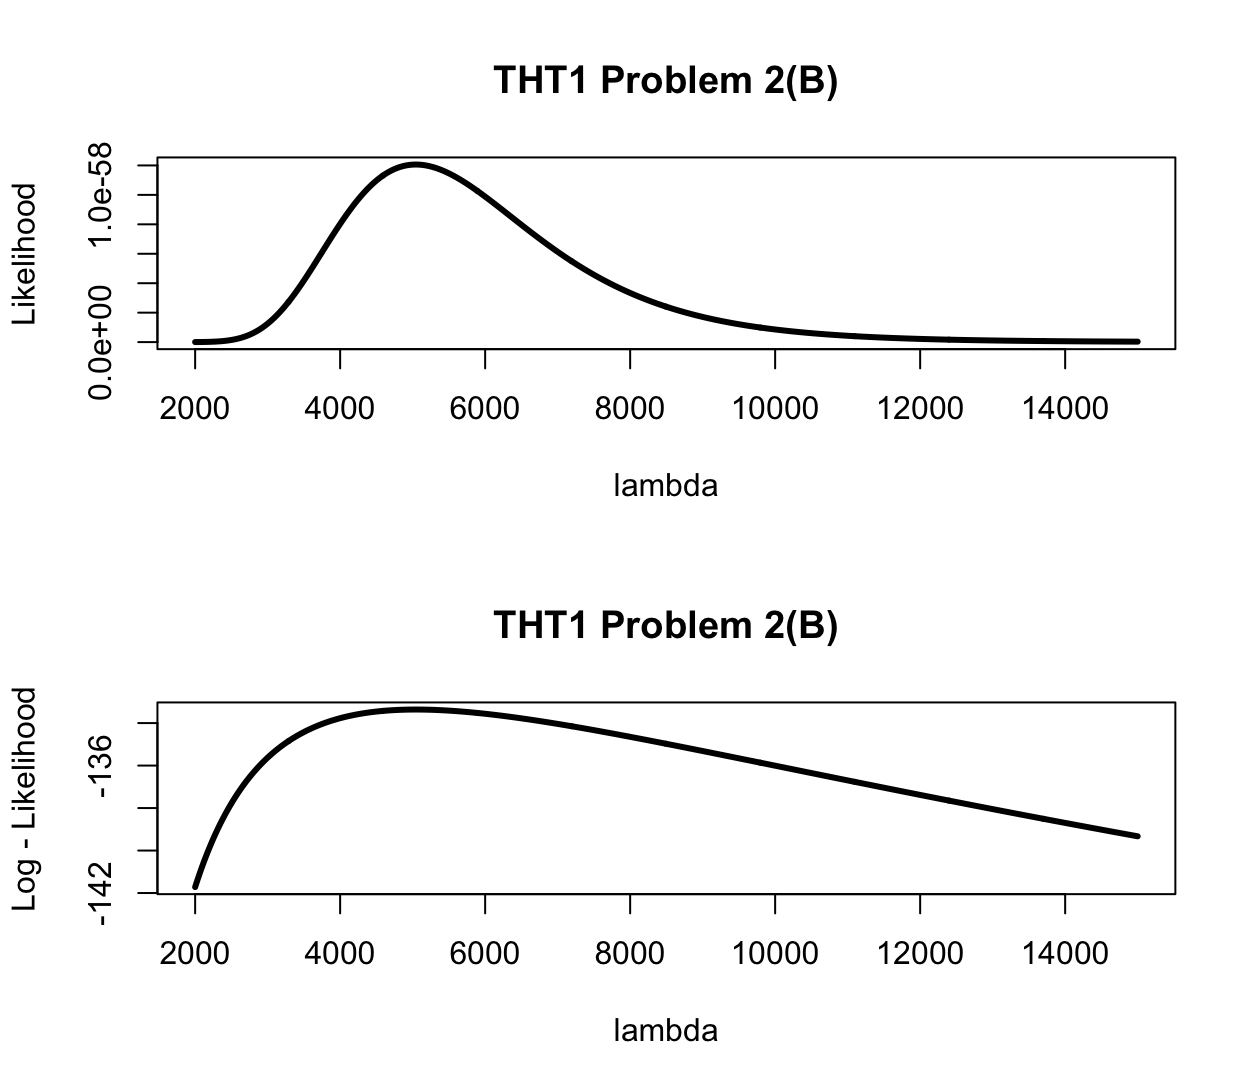
\includegraphics[scale = .3]{THT12Bii}\]
        From inspection of our log-likelihood graph we can see that $\hat{y}( = 5043.71)$ yields the maximum value meaning it is sufficient for $\lambda$ in the Exponential sampling model. 

        Let us now take the derivative of our log-likelihood function with respect to $\lambda$,
        \[\frac{d}{d\lambda}ll(\lambda \given \undertilde{y}\bm{E}) = -\frac{n}{\lambda} + \frac{s}{\lambda^{2}}\]

        Now solving for when this is 0, we get that,
        \begin{align*}
            -\frac{n}{\lambda} + \frac{s}{\lambda^{2}} = 0 \Longleftrightarrow& \frac{n}{\lambda} = \frac{s}{\lambda^{2}} \\
            \Longleftrightarrow& \lambda = \hat{\lambda}_{MLE} = \frac{s}{n} = \hat{y}_n = 5043.71
        \end{align*}

        \[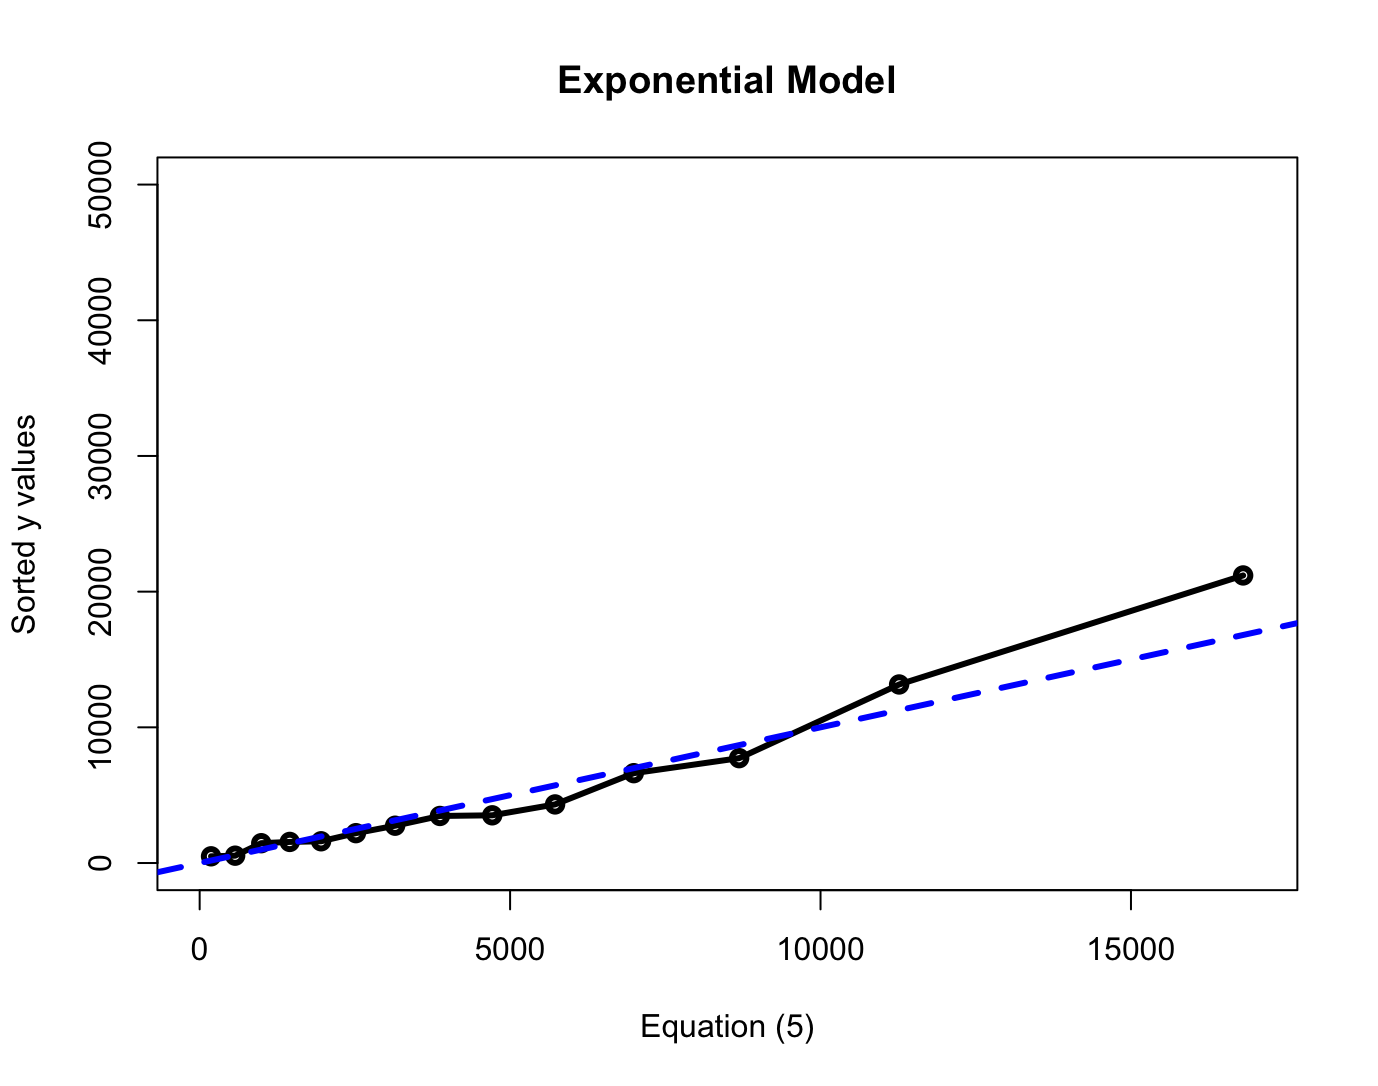
\includegraphics[scale = .25]{THT12Bii(5)}\]

        Since the target shape is the $45^{\circ}$ line, most the values seem pretty close to that mark, and the only potential outliers seems to be the last data value. We see with Monte Carlo that it is well within the uncertainty bands.
        \[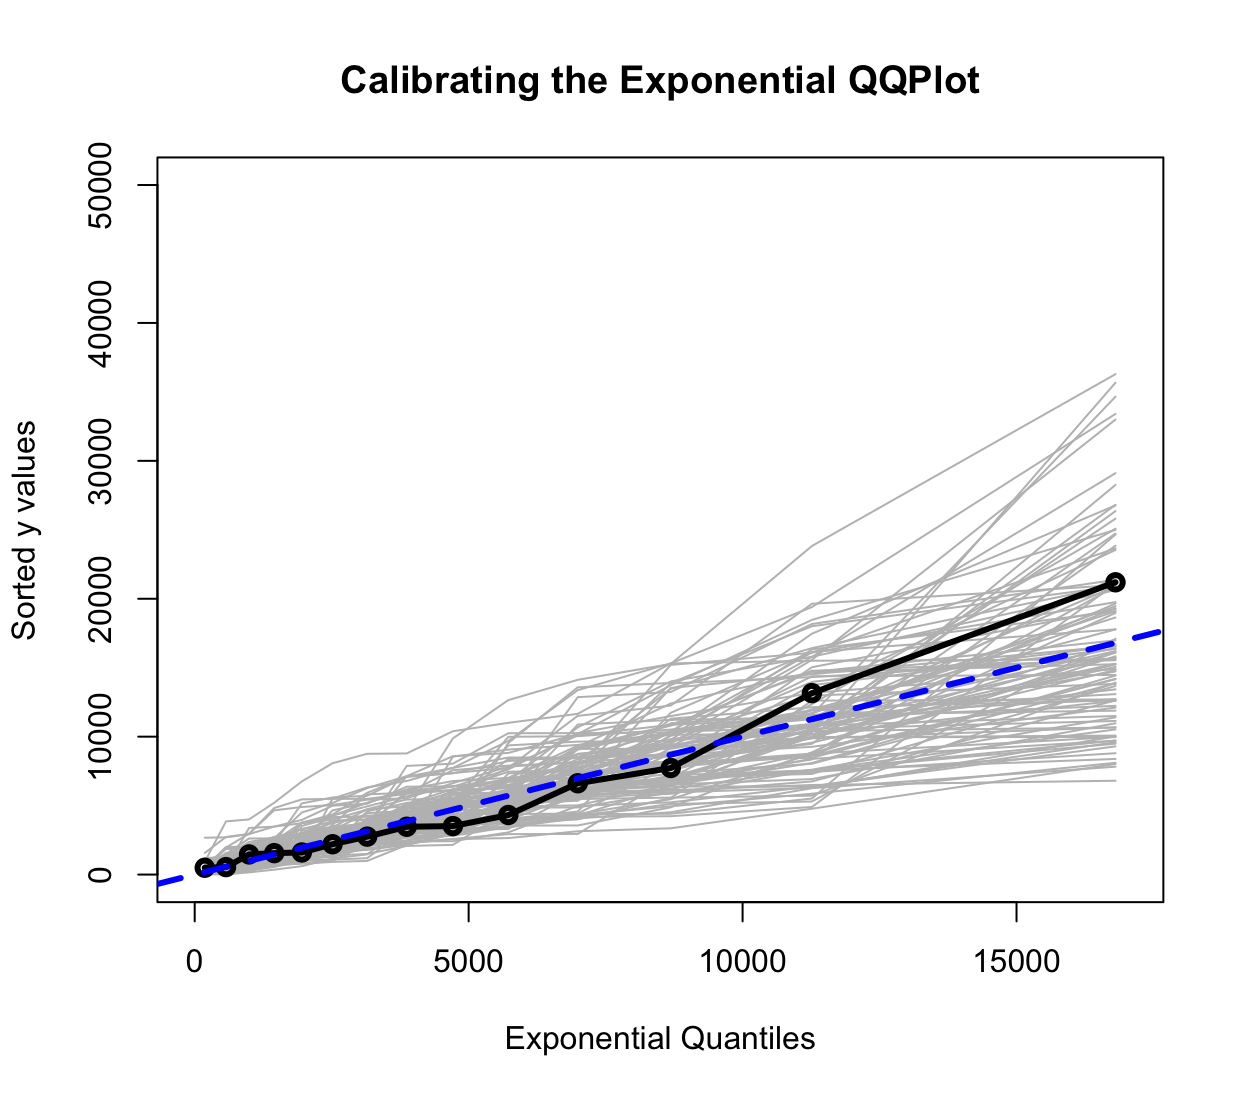
\includegraphics[scale = .26]{bands}\]
    \end{solution}
\end{tcolorbox}

\end{itemize}
\vspace{0.5in}
\item[(ii)]By regarding Your likelihood in 2(B)(i)(b) as an unnormalized probability density function for $\lambda$, show that the conjugate family for the Exponential$( \lambda )$ likelihood (parameterized as in (\ref{e:exponential-model-1})) is the set of \textit{Inverse Gamma} distributions $\Gamma^{ -1 } ( \alpha, \beta )$ for $\alpha > 0, \beta > 0$ (\textbf{NB} $W \sim \Gamma^{ -1 } ( \alpha, \beta )$ just means that $\frac{ 1 }{ W } \sim \Gamma ( \alpha, \beta )$; see Table A.1 in Appendix A in Gelman et al.~(2014)):
\begin{equation} \label{e:inverse-gamma-1}
\lambda \sim \Gamma^{ -1 } ( \alpha, \beta ) \ \ \ \iff \ \ \ p ( \lambda \given \bm{ IG } ) = \left\{ \begin{array}{cc} \frac{ \beta^\alpha }{ \Gamma ( \alpha ) }
\lambda^{ - ( \alpha + 1 ) } \exp \left( - \frac{ \beta }{ \lambda } \right)
& \textrm{for } \lambda > 0 \\ 0 & \mbox{otherwise} \end{array} \right\} \, ,
\end{equation}
in which $\bm{ IG }$ stands for the Inverse Gamma sampling distribution assumption \textit{[5 points]}.
\begin{tcolorbox}[breakable]
    \begin{solution}
        We see that our likelihood function,
        \[l(\lambda \given \undertilde{y}\bm{E}\mathcal{B}) = C_+\lambda^{-n}\exp(-\frac{s}{n})\] actually is part of the Inverse Gamma Distributions.
        \[P(\lambda \given \alpha \beta) = C_+\lambda^{-(\alpha + 1)} \exp(-\frac{\beta}{\lambda})\]
    \end{solution}
\end{tcolorbox}

\vspace{0.5in}

\item[(iii)]

By directly using Bayes's Theorem (and ignoring constants), show that
the prior-to-posterior updating rule in this model is
\begin{equation} \label{e:updating-1}
\left\{ \begin{array}{ccc} ( \lambda \given \bm{ IG } )& \sim & \Gamma^{ -1 } ( \alpha, \beta )
\\ ( Y_i \given \lambda \, \bm{ E } \, \mathcal{ B } ) & \stackrel{ \mbox{\tiny IID} }{ \sim } & \textrm{Exponential} ( \lambda ) \end{array} \right\} \Longrightarrow ( \lambda \given \bm{ y } \, \bm{ IG } \, \bm{ E } \, \mathcal{ B } ) \sim \Gamma^{ -1 } ( \alpha + n, \beta + n \bar{ y } ) \, ,
\end{equation}
where $\bm{ y } = ( y_1, \dots, y_n )$. \textit{[10 points]}
\begin{tcolorbox}[breakable]
    \begin{solution}
        Consider the following,
        \begin{align*}
            P(\lambda \given \bm{y}\, \bm{IG} \, \bm{E} \mathcal{B}) &= C_+ \left[C_+\lambda^{-(\alpha + 1)}\exp\left(-\frac{\beta}{\lambda}\right)\right]\cdot \left[C_+ \lambda^{-n}\exp\left(-\frac{s}{\lambda}\right)\right] \\
            &= C_+ \lambda^{-(\alpha + n )-1}\exp\left(-\frac{\beta + s}{\lambda}\right) \\
            &= \Gamma^{-1}(\alpha+n, \beta + s) \\
            &= \Gamma^{-1}(\alpha+n, \beta + n\bar{y})
        \end{align*}
        Meaning $( \lambda \given \bm{ y } \, \bm{ IG } \, \bm{ E } \, \mathcal{ B } ) \sim \Gamma^{ -1 } ( \alpha + n, \beta + n \bar{ y } )$
    \end{solution}
\end{tcolorbox}

\newpage
\item[(iv)]

It turns out that the mean and variance of the $\Gamma^{ -1 } (
\alpha, \beta )$ distribution are $\frac{ \beta }{ \alpha - 1}$ (when $\alpha > 1$) and $\frac{ \beta^2 }{ ( \alpha - 1 )^2 ( \alpha - 2 ) }$ (as long as
$\alpha > 2$), respectively. Use this to write down an explicit formula showing that the posterior mean is a weighted average of the prior and sample means, and
conclude from this formula that $n_0 = ( \alpha - 1 )$ is the prior effective
sample size. Note also from the formula for the likelihood in this problem
that, when thought of as a distribution in $\lambda$, it's equivalent to a
constant times the $\Gamma^{ -1 } ( n - 1, n \, \bar{ y } )$ distribution. \textit{[10 points]} 
\begin{tcolorbox}[breakable]
    \begin{solution}
        Well we know from above that we have the posterior $\alpha$ and $\beta$ to be,
        \begin{align*}
            \alpha_{\text{posterior}} = \alpha + n && \beta_{\text{posterior}} = \beta + n\bar{y}
        \end{align*} 
        meaning out posterior mean will be,
        \[\frac{\beta + n\bar{y}}{\alpha + n - 1}\]
        and as a reminder we have our prior mean as $\dfrac{\beta}{\alpha - 1}$ and sample mean as $\dfrac{s}{n}$, so to show the posterior mean is a weighted average of the prior and sample mean, we have to solve for $w_1$ and $w_2$ that satisfy the following,
        \[\frac{\beta + n\bar{y}}{\alpha + n - 1} = w_1 \left(\frac{\beta}{\alpha -1 }\right) + w_2 \left(\frac{s}{n}\right).\]
        We see though through $w_1 = \dfrac{\alpha-1}{\alpha- 1 + n}$ and $w_2 = \dfrac{n}{\alpha -1 + n}$ we satisfy the above,
        \begin{align*}
            \dfrac{\alpha-1}{\alpha- 1 + n}\left(\frac{\beta}{\alpha -1 }\right) + \dfrac{n}{\alpha -1 + n}\left(\frac{s}{n}\right)&= \dfrac{\beta}{\alpha -1 + n} + \dfrac{s}{\alpha -1 + n} \\
            &= \dfrac{\beta + s}{\alpha -1 + n} \\
            &= \dfrac{\beta + n \bar{y}}{\alpha -1 + n}
        \end{align*}
        as desired. Next we see that our data sample size is the numerator of $w_2$ and thus $n_0 = (\alpha -1)$ is the prior effective sample size.
    
        We have our likelihood function as, $l(\lambda \given \undertilde{y}\bm{E}\mathcal{B}) = C_+ \lambda^{-n}\exp\lrp{-\dfrac{s}{n}}$, and the inverse gamma function is $\Gamma^{-1} = C_+\lambda^{-(\alpha + 1)}\exp\lrp{-\dfrac{\beta}{\lambda}}$, we see then that $\alpha = n -1$ and $\beta = s$ meaning it is the distribution $\Gamma^{-1}(n-1, s) = \Gamma^{-1}(n-1, n\bar{y})$.
    \end{solution}
\end{tcolorbox}


\newpage

\item[(v)]

The researcher from EEE has prior information from another experiment she judges to be comparable to this one: from this other experiment the prior for $\lambda$ should have a mean of about $\mu_0 =$ 4,500 and an SD of about $\sigma_0 =$ 1,800.  

\begin{itemize}

\item[(a)] 

Show that this corresponds to a $\Gamma^{ -1 }( \alpha_0, \beta_0 )$
prior with $( \alpha_0, \beta_0 ) = ( 8.25, 32625 )$, and therefore to a
prior sample size of about 7. Is this amount of prior information small, medium or large in the context of her data set? Explain briefly. \textit{[10 points]}
\begin{tcolorbox}
    \begin{solution}
        We have,
        \begin{align*}
            \text{prior mean} &= \mu_0 = 4500 = \dfrac{\beta_0}{\alpha_0 - 1} \\
            \text{prior SD} &= \sigma_0 = 1800 \\
            \text{prior variance } &= \sigma_0^{2} = 1800^{2} = \dfrac{\beta_0^{2}}{(\alpha_0 -1)^{2}(\alpha_0-2)}
        \end{align*}
        this gives us the system of equations,
        \begin{align*}
            \mu_0 = \dfrac{\beta_0}{\alpha_0 -1} && \sigma_2 = \dfrac{\beta_0^{2}}{(\alpha_0-1)^{2}(\alpha_0 -2)}
        \end{align*}
        where solving for $(\alpha_0, \beta_0)$ gives us,
        \begin{align*}
            \alpha_0 = \dfrac{\mu_0^{2} + 2\sigma_0^{2}}{\sigma_0^{2}} && \beta_0 = \dfrac{\mu_0(\mu_0^{2} + \sigma_0^{2})}{\sigma_0^{2}}
        \end{align*}
        finally plugging in our $(\mu_0, \sigma_0) = (4500, 1800)$ we get $(\alpha_0,\beta_0) = (8.25, 32625)$. Since our prior effective sample size was $n_0 = (\alpha -1)$ plugging in our $\alpha_0$ we get about 7. This is amount of prior information is about medium in the context of her data set, because she has a data set of size 14. 
    \end{solution}
\end{tcolorbox}


\newpage
\item[(b)] 

Thinking of each of the prior, likelihood and posterior densities as Inverse Gamma distributions, work out the SDs of each of these information sources, and numerically summarize 	the updating from prior to posterior by completing Table \ref{t:prior-likelihood-posterior} (show Your work) \textit{[10 points]}.
\begin{tcolorbox}[breakable]
    \begin{solution}
        If we think of the prior, likelihood, and posterior densities as Inverse Gamma distributions they would explicitly be, 
        \[\Gamma^{-1}(\alpha_0, \beta_0), \ \Gamma^{-1}(n-1, s), \ \Gamma^{-1}(\alpha_0 + n, \beta_0 + s)\]
        respectively. Next we know that the the expected value of $\lambda$ given Inverse Gamma, $\alpha$, and $\beta$ is,
        \[E(\lambda \mid \Gamma^{-1}\alpha,\beta)\]
        We know the variance to be,
        \[V(\gamma \mid \Gamma^{-1}\alpha\beta) = \frac{\beta^{2}}{(\alpha -1)^{2}(\alpha -2)}\]
        and because $\beta > 2$ and we are picking $\alpha > 2$ we can take the square root of the variance to get the standard deviation without worry of imaginary answers,
        \[SD(\lambda \mid \Gamma^{-1}\alpha \beta) = \frac{\beta}{(\alpha - 1)\sqrt{\alpha - 2}}\]
    
        We know our prior inputs to be $(\alpha,\beta) = (\alpha_0,\beta_0) = (8.25, 32,625)$ and plugging this into the above equations (used R) we get the prior mean to be 4500 and the prior standard deviation to be 1800
    
        Our likelihood inputs were $(\alpha, \beta) = (n-1,s) = (14 -1, 70612)$ plugging this in again (used R) we get our likelihood mean and likelihood standard deviation to be 5884.333 and 1774.193 respectively. 
    
        Finally our posterior inputs were $(\alpha, \beta) = (\alpha_0 + n, \beta + s) = (22.25, 103,237)$ so plugging this in one more time (used R) we get our posterior mean and standard deviation to be 4858.212 and 1079.603 respectively. 
    \end{solution}
\end{tcolorbox}


\bigskip

\begin{table}[t!]

\centering

\caption{\textit{Bayesian updating in the wire-failure case study.}}

\label{t:prior-likelihood-posterior}

\bigskip

\begin{tabular}{c|ccc}

\multicolumn{1}{c}{} & \multicolumn{3}{c}{$\lambda$} \\ \cline{2-4}

\multicolumn{1}{c}{} & Prior & Likelihood & Posterior \\

\hline

Mean & 4,500 & 5884& 4,858 \\

SD & 1800& 1,774 & 1080 \\

\end{tabular}

\end{table}

\bigskip
\newpage
\item[(c)] 

Make a plot of the prior, likelihood and posterior distributions on the same graph (with $\lambda$ ranging on the horizontal scale from 1,000 to 12,000), identifying which curve corresponds to which density (You can use the \texttt{R} code on the course web page for the Inverse Gamma density function, or You can write Your own code to evaluate the density in equation (\ref{e:inverse-gamma-1})). In what sense, if any, is the posterior a compromise between the prior and likelihood? Explain briefly. \textit{[15 points]}
\begin{tcolorbox}[breakable]
    \begin{solution}
        \[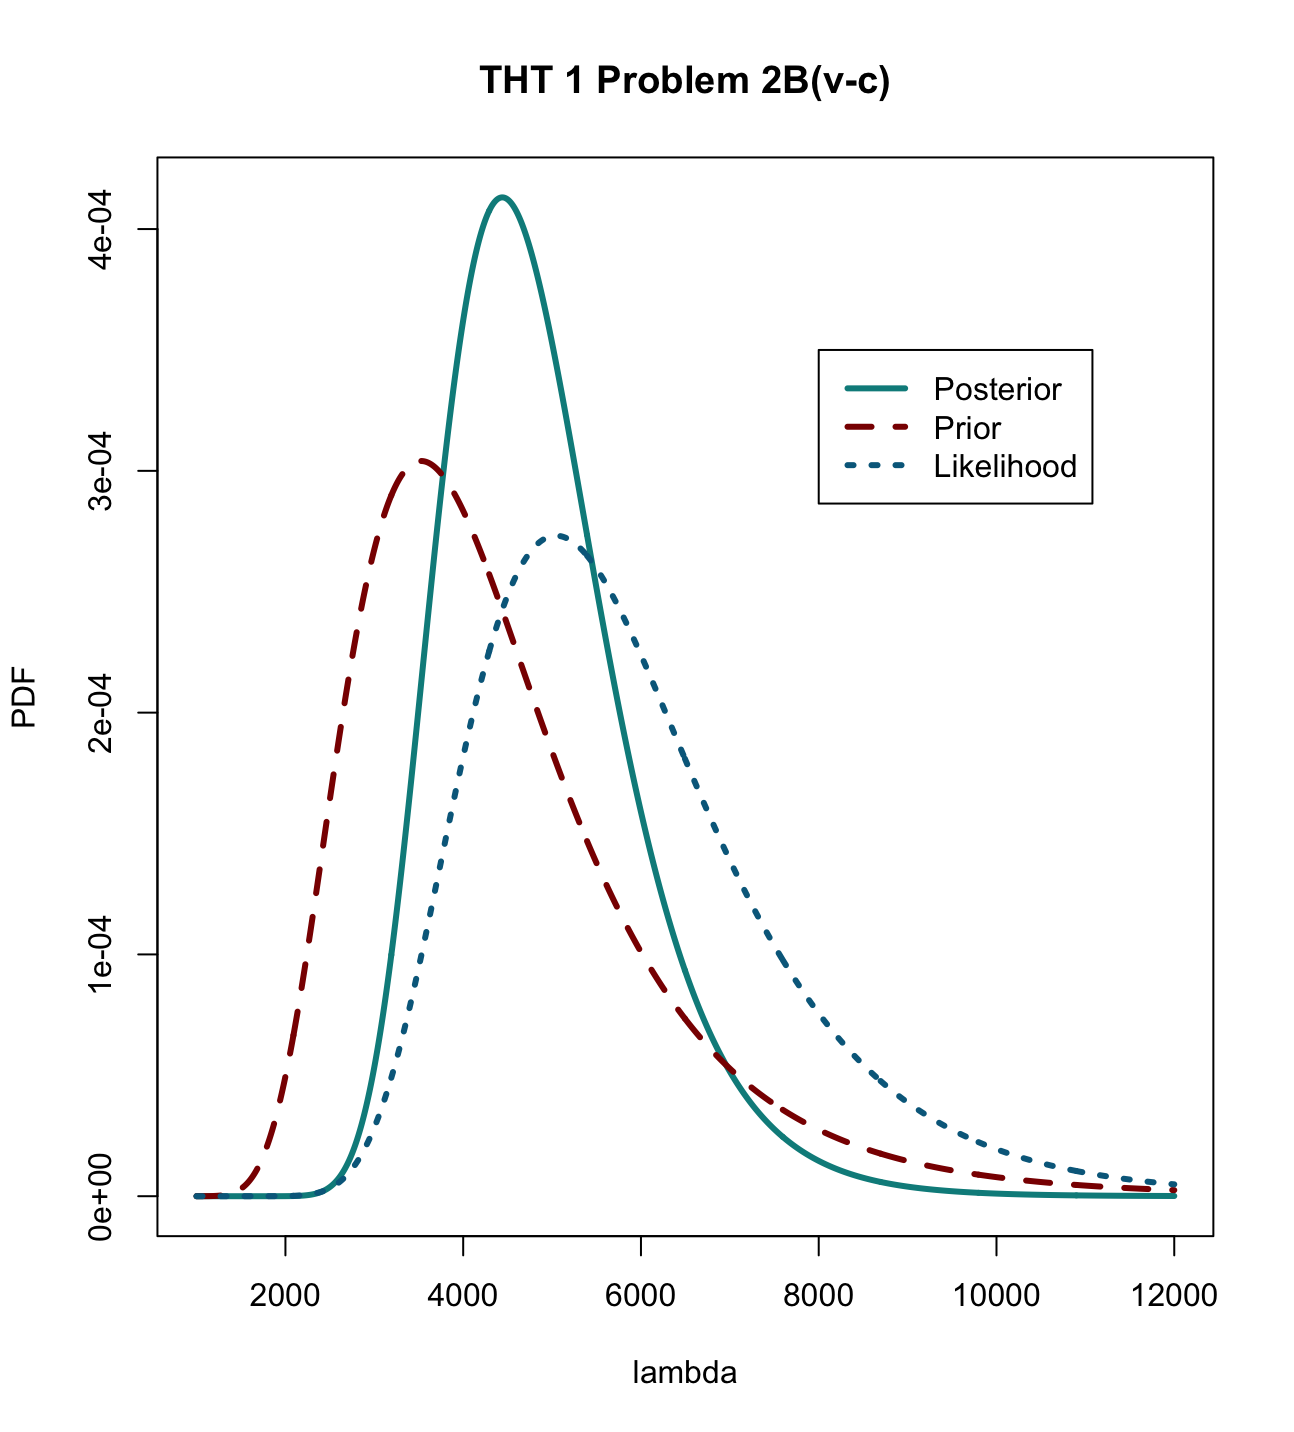
\includegraphics[scale = 0.25]{THT12bvc.png}\]
        We see that it is indeed a compromise by being the in the center of the prior and likelihood PDF, it also has more information of than the other to, which we see through the height of its peak compared to the other two. 
    \end{solution}
\end{tcolorbox}

\newpage
\item[(d)] 

Compute the observed information with this data set, and use this to compute an estimated standard error for the MLE and construct an approximate 99.9\% frequentist confidence interval for $\lambda$. Use the \texttt{qgamma} function in \texttt{R} (or some other numerical integration routine of Your choice) to work out the left and right endpoints of the 99.9\% central posterior interval for $\lambda$ (\textit{Hint:} Remember the \textbf{NB} in 2(B)(ii)), and compare with the frequentist interval. Give two reasons why they're so different in this problem. Is one of them ``right'' and the other one ``wrong','' or are they trying to summarize different amounts and types of information, or what? Explain briefly. \textit{[25 points]}
\begin{tcolorbox}[breakable]
    \begin{solution}
        First we will have to take the likelihood function which to recall is,
        \[l(\lambda \mid \undertilde{y}\bm{E}\mathcal{B}) = C_+ \lambda^{-n}\exp(-\frac{s}{\lambda})\]
        and consider take the log of it to get the log-likelihood function which was,
        \[ll(\lambda\mid \undertilde{y}\bm{E}\mathcal{B}) = C_+ - n\log(\lambda) - \dfrac{s}{n}\]
        and now we take the first derivative of the log-likelihood function with respect to lambda,
        \[\dfrac{d}{d\lambda}ll(\lambda\mid \undertilde{y}\bm{E}\mathcal{B}) = -\dfrac{n}{\lambda} + \dfrac{s}{\lambda^{2}}.\]
    
        Now from here we can are able to maximize the log-likelihood function, but simply setting the derivate we took above to 0 and solving for $\lambda$,
        \begin{align*}
            -\dfrac{n}{\lambda} + \dfrac{s}{\lambda^{2}} &= \dfrac{-n\lambda + s}{\lambda^{2}} = 0 \\
            s &= n\lambda \\
            \dfrac{s}{n} &= \lambda 
        \end{align*}
        Meaning $\lambda_{MLE} = \lambda = \dfrac{s}{n} = \bar{y_n}$. Next to compute the observed information we must take the 2nd derivative of the log-likelihood function which works out to be,
        \[\dfrac{d^{2}}{d^{2}\lambda^{2}}ll(\lambda \mid \undertilde{y}\bm{E}\mathcal{B}) = \dfrac{d}{d\lambda}\lrp{-n\lambda^{-1} + s\lambda^{-2}} = n\lambda^{-2} -2s\lambda^{-3}\]
        With this we can compute the observed information,
        \begin{align*}
            \hat{I}(\hat{\lambda}_{MLE}) &= \lrb{-\dfrac{d^{2}}{d\lambda^{2}} ll(\lambda \mid \undertilde{y}\bm{E}\mathcal{B})}_{\lambda = \lambda_{MLE}} \\ &=\lrb{-\dfrac{n}{\lambda^{2}} +\dfrac{2s}{\lambda^{3}}}_{\lambda = \lambda_{MLE}} \\
            &= -\dfrac{n}{\lrp{\dfrac{s}{n}}^{2}} + \dfrac{2s}{\lrp{\dfrac{s}{n}}^{3}} \\
            &= -\dfrac{n^{3}}{s^{2}} + \dfrac{2sn^{3}}{s^{3}} \\
            &= \dfrac{n^{3}}{s^{2}} \\
            &= n\cdot \lrp{\dfrac{s}{n}}^{-2} = n\lambda_{MLE}^{-2} = \dfrac{n}{\lambda_{MLE}^{2}} = 5.503349\cdot 10^{-7}
        \end{align*}
    
        Now to compute an estimated standard error, we know it is simply the square root of the estimated variance for the MLE, which we know is,
        \[\hat{V}_{IID}(\hat{\lambda}_{MLE}) = \lrb{\hat{I}(\hat{\lambda}_{MLE})}^{-1} = \dfrac{\hat{\lambda}_{MLE}}{n} = 1817075\]
        meaning our estimated standard error is simply, 
        \[\hat{SE}_{IID}(\hat{\lambda}_{MLE}) = \sqrt{\hat{V}_{IID}(\hat{\lambda}_{MLE}) } = 1347.189\]
        Finally to construct our $100(1-\alpha')\%$ CI (where here our $\alpha' = 0.001$) it is simply,
        \[\hat{\lambda }_{MLE} \pm \Phi^{-1}(1 - \frac{\alpha'}{2})\hat{SE}(\hat{\lambda}_{MLE})\]
        So plugging in all our values that we worked out (used R) we get,
        \begin{align*}
            99.9\%CI = 5043.714 \pm 3.2905\cdot 1347.99 = (608.1193, 9479.3093)
        \end{align*}
    
        Now to compare it with the posterior interval we will use the inverse gamma function to obtain the interval end points. Recalling our posterior $\alpha$ to be our prior $\alpha$ summed with $n$, and our posterior $\beta$ to be the sum of the prior $\beta$ and $s$, and we the end points of the interval to be at $\dfrac{\alpha'}{2}$ and $1 - \dfrac{\alpha'}{2}$ where $\alpha' = 0.001$. Once we plug this into R we obtain the interval to be,
        \[(2511.783, 10423.188)\]
    
        Neither of them are right or wrong, it is the 3rd explanation in that they are summarizing different amounts and types of information. The posterior interval is taking into account the prior information, which we deemed to be medium to high, alongside the likelihood information. While the frequentist interval is simply taking the likelihood information or in other words just the data in front of us. Basically it boils down to the posterior interval accounting for the prior and the likelihood, while the frequentist interval is simply the likelihood. 
    \end{solution}
\end{tcolorbox}


\end{itemize}

\end{itemize}

\end{itemize}

\newpage
\textbf{CODE FOR PROBLEMS}
\begin{lstlisting}[language = R]
#PROBLEM 2A-iv ============================================   
ppv_v <- rep(0,11)
npv_v <- rep(0,11)
alpha_v <- rep(0,11)

PPV <- function(alpha, beta, gamma) {
  ppv <- (alpha * beta)/((alpha * beta) + (1 - alpha)*(1-gamma))  
  return(ppv)
}

NPV <- function(alpha, beta, gamma) {
  npv <- (gamma * (1- alpha)) / (alpha * (1-beta) + (1-alpha)*gamma)
  return(npv)
}
  
alpha_star <- 0.00286
beta <- 0.99
gamma <- 0.95

alpha_star_points <- 1000
alpha <- seq(0, 10 *alpha_star, length = alpha_star_points)
plot(alpha, NPV(alpha, beta, gamma), type = 'l', 
    lwd = 3, col = 'darkcyan', ylab = 'NPV', ylim = 0:1)
title(main = "THT1 2(A)(iv) NPV", col.main="red", font.main = 4)
#END PROBLEM 2A-iv ============================================  
\end{lstlisting}

\begin{lstlisting}
#2B-i-b ================================================

#LIKELIHOOD AND LOG-LIKELIHOOD PLOTS====================
y <- c(495, 541, 1461, 1555, 1603, 2201, 
2750, 3468, 3516, 4319, 6622, 7728, 13159, 21194)
lambda.hat <- mean(y)
print(s <- sum( y ))

exponential.likelihood <- function(lambda, y) {
   n <- length( y )
   s <- sum( y )
   ell <- lambda^( -n ) * exp(-s/lambda)
   return(ell)
}

lambda.grid <- seq(2000,15000, length = 1000)
par( mfrow = c(2,1))
plot(lambda.grid, exponential.likelihood(lambda.grid, y), 
    type = 'l', lwd =3 ,main = 'THT1 Problem 2(B) ii ', 
    ylab = 'Likelihood', xlab = 'lambda')


exponential.log.likelihood <- function(lambda, y) {
  n <- length( y )
  s <- sum( y )
  ell.ell <- -n*log(lambda) - s/lambda
  return(ell.ell)
}

plot(lambda.grid, exponential.log.likelihood(lambda.grid, y), 
    type = 'l', lwd =3 ,main = 'THT1 Problem 2(B) ii', 
    ylab = 'Log - Likelihood', xlab = 'lambda')

par( mfrow = c(1,1))
#END - LIKELIHOOD AND LOG-LIKELIHOOD PLOTS==============


#EXPONENTIAL MODEL PLOT AGAINST 45 degree line =========
y <- c(495, 541, 1461, 1555, 1603,
 2201, 2750, 3468, 3516, 4319, 
 6622, 7728, 13159, 21194)
lambda.hat <- mean(y)

F.inverse <- function(lambda, p) {
  result <- -lambda * log(1 - p)
  return(result)
}

plot(0,0,
     xlab = 'Equation (5)', ylab = 'Sorted y values',
     main = 'Calibrating the Exponential QQPlot',
     xlim = c(0, 17000), type = 'n', ylim = c(0, 50000),
     title = 'Exponential Model')


lines(F.inverse(lambda.hat, ((1:14) - .5) /14 ), 
y, type = 'o', xlim = c(0,max(y)), lwd = 3)

abline(0,1, lwd = 3, col = 'blue', lty = 2)    
#END - EXPONENTIAL MODEL PLOT AGAINST 45 degree line =========

#CALIBRATING QQPLOT =========================================
y <- c(495, 541, 1461, 1555, 1603, 2201, 
2750, 3468, 3516, 4319, 6622, 7728, 13159, 21194)
lambda.hat <- mean(y)

F.inverse <- function(lambda, p) {
  result <- -lambda * log(1 - p)
  return(result)
}

plot(0,0,
     xlab = 'Exponential Quantiles', ylab = 'Sorted y values',
     main = 'Calibrating the Exponential QQPlot',
     xlim = c(0, 17000), type = 'n', ylim = c(0, 50000))

n <- 14
M <- 100

for (i in 1:M) {
  y.star <- sort( rexp(n, 1 / lambda.hat) )
  lines( F.inverse(lambda.hat, ( (1:n) -0.5)/n), y.star, 
    lwd = 1, col = 'gray')
}

lines(F.inverse(lambda.hat, ((1:14) - .5) /14 ), y, 
    type = 'o', xlim = c(0,max(y)), lwd = 3)

abline(0,1, lwd = 3, col = 'blue', lty = 2)
#END CALIBRATING QQPLOT =====================================

#END -2B-i-b ================================================

#2B-V-c======================================================
y <- c( 495, 541, 1461, 1555, 1603, 2201, 2750, 3468, 3516, 4319, 6622, 
        7728,
        13159, 21194 )

n <- length( y )
s <- sum( y )

theta <- seq(.10, .25, length = 4000)

inverse.gamma.mean <- function(a, b) {
  mean <- b / (a-1)
  
  return(mean)
}

inverse.gamma.sd <- function(a,b) {
  sd <- b / ((a-1)* sqrt(a-2))
  
  return(sd)
}


alpha.prior <- 8.25
beta.prior <- 32625

alpha.posterior <- 22.25
beta.posterior <- 103237

alpha.likelihood <- 13
beta.likelihood <- s

lambda.mle <- s/n
info <- n / (lambda.mle^2)
variance.lambda <- info^-1



lambda.grid <- seq(1000,12000, length = 1000)

print( p.n.summary <- c(inverse.gamma.mean(22.25, 103237), 
    inverse.gamma.sd(22.25, 103237)))
no.underflow.or.overflow.inverse.gamma.pdf <-
  function( lambda, alpha, beta ) {
    #   to make the function crash-proof, need to put in
    #   some logical language to check that lambda > 0,
    #   alpha > 0, and beta > 0; i won't do this here
    log.pdf.value <- alpha * log( beta ) - lgamma( alpha ) -
      ( alpha + 1 ) * log( lambda ) - beta / lambda
    return( exp( log.pdf.value ) )
  }
lambda.grid <- seq( 1000, 12000, length = 1000 )
plot( lambda.grid, no.underflow.or.overflow.inverse.gamma.pdf( 
  lambda.grid,
  alpha.posterior, beta.posterior ), type = 'l', lwd = 3, lty = 1,
  xlab = 'lambda', ylab = 'PDF', main = 'THT 1 Problem 2B(v-c)',
  col = 'darkcyan' )

lines( lambda.grid, no.underflow.or.overflow.inverse.gamma.pdf( 
  lambda.grid,
  alpha.prior, beta.prior ), lwd = 3, lty = 2, col = 'darkred' )
lines( lambda.grid, no.underflow.or.overflow.inverse.gamma.pdf( 
  lambda.grid,
  alpha.likelihood, beta.likelihood ), lwd = 3, lty = 3, col = 
    'deepskyblue4' )
legend( 8000, 3.5e-04, 
    legend = c( 'Posterior', 'Prior', 'Likelihood' ),
    lty = c( 1, 2, 3 ), lwd = c( 3, 3, 3 ), 
    col = c( 'darkcyan','darkred', 'deepskyblue4' ) )


#END-2B-V-c======================================================

#2B-V-d==========================================================
library(invgamma)
y <- c( 495, 541, 1461, 1555, 1603, 2201, 2
    750, 3468, 3516, 4319, 6622, 7728, 13159, 21194 )

n <- length( y )
s <- sum( y )

alpha.prior <- 8.25
beta.prior <- 32625

alpha.posterior <- 22.25
beta.posterior <- 103237

alpha.likelihood <- 13
beta.likelihood <- s

lambda.mle <- s/n
info <- n / (lambda.mle^2)
variance.lambda <- info^-1

SE.lambda <- sqrt(variance.lambda)

z.magicnumber <- qnorm(1- (0.001/2))


#Frequentist Interval
CI <- c(lambda.mle - z.magicnumber*SE.lambda, 
    lambda.mle + z.magicnumber*SE.lambda)

print(CI)

#Bayesian Interval
bayesian.interval <- c(qinvgamma(0.001/2, alpha.posterior, 
    beta.posterior), 
    qinvgamma(1-(0.001/2), alpha.posterior, beta.posterior))

print(bayesian.interval)
#END-2B-V-d======================================================
\end{lstlisting}

\begin{lstlisting}[language = R]
#PROBLEM 2B-V-D ============================================    
library(invgamma)
n <- 14
s <- 32625
alpha.prior <- 8.25
beta.prior <- 32625
alpha.posterior <- alpha.prior + n
beta.posterior <- 103237
alpha.likelihood <- 13
beta.likelihood <- s

lambda.mle <- s/n
info <- n / (lambda.mle^2)
variance.lambda <- info^-1

SE.lambda <- sqrt(variance.lambda)

z.magicnumber <- qnorm(1- (0.001/2))

#Frequentist interval
CI <- c(lambda.mle - z.magicnumber*SE.lambda, 
    lambda.mle + z.magicnumber*SE.lambda)

print(CI)
print(SE.lambda)

bayesian.interval <- 
    c(qinvgamma(0.001/2, alpha.posterior, beta.posterior), 
    qinvgamma(1-(0.001/2), alpha.posterior, beta.posterior))
print(bayesian.interval)
#END PROBLEM 2B-V-D ========================================
\end{lstlisting}

\end{document}
